\section{Entendimento do Fluxo Antigo}

Antes do desenvolvimento do módulo, as solicitações de mudanças de categoria eram realizadas por meio de correio eletrônico. Após o recebimento do pedido, a alteração dependia da intervenção de um membro da equipe responsável, que executava manualmente as operações necessárias diretamente no banco de dados por meio de uma QUERY SQL reutilizável.

Esse procedimento estabelece uma dependência entre a solicitação do especialista e a disponibilidade de um responsável com acesso técnico à base de dados. Além disso, o acompanhamento do pedido e a consulta ao histórico das alterações dependiam dos registros e das comunicações existentes fora de um fluxo centralizado e auditável na aplicação.

\begin{figure}[htbp]
    \centering
    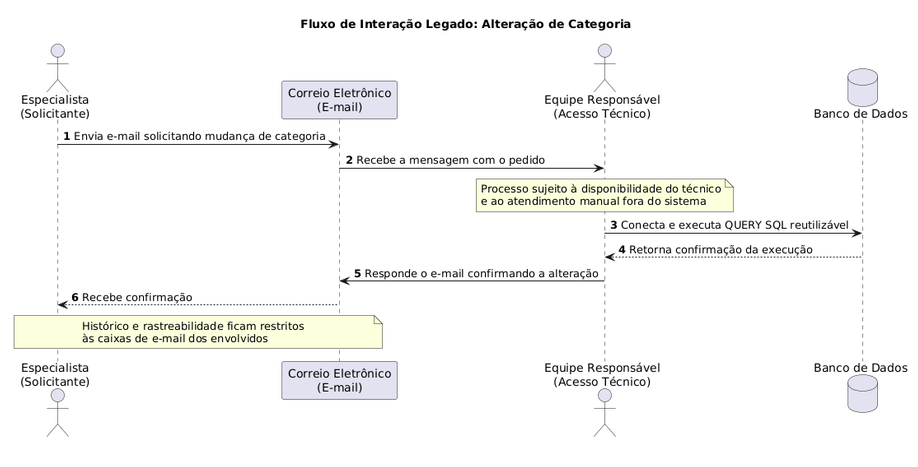
\includegraphics[width=0.8\textwidth]{dados/figuras/old_workflow.png}
    \caption{Fluxo de alteração de categoria de especialistas antes do desenvolvimento do módulo.}
\end{figure}

A análise desse processo permitiu identificar a necessidade de incorporar ao sistema mecanismos para registrar as solicitações, formalizar as decisões e acompanhar as alterações realizadas.
